% Intended LaTeX compiler: xelatex
\documentclass[10pt, svgnames]{beamer}
\usepackage{graphicx}
\usepackage{longtable}
\usepackage{wrapfig}
\usepackage{rotating}
\usepackage[normalem]{ulem}
\usepackage{amsmath}
\usepackage{amssymb}
\usepackage{capt-of}
\usepackage{hyperref}
\usetheme{metropolis}
\author{Sappinandana Akamphon}
\date{\today}
\title{Introduction to Engineering Design}
\subtitle{ME 310: Mechanical Design}
\usepackage{booktabs}
\usepackage{pgfplots}
\usepackage{multirow}
\usepackage{smartdiagram}
\pgfplotsset{compat=1.18}
\definecolor{lightblue}{RGB}{180,220,255}
\institute{Department of Mechanical Engineering, TSE}
\date{}
\usetikzlibrary{patterns,shapes,arrows}
\AtBeginSection[]{\begin{frame}{Outline}\tableofcontents[currentsection]\end{frame}}
\hypersetup{
 pdfauthor={Sappinandana Akamphon},
 pdftitle={Introduction to Engineering Design},
 pdfkeywords={},
 pdfsubject={},
 pdfcreator={Emacs 30.0.50 (Org mode 9.6)}, 
 pdflang={English}}
\begin{document}

\maketitle

\section{Basic Types of Loads and Stresses}
\label{sec:orgd0e4183}
\begin{frame}[label={sec:org7f43aaa}]{What to Consider in Load Types}
\begin{itemize}
\item Stresses
\item Deformation
\end{itemize}
\end{frame}

\begin{frame}[label={sec:org52578c8}]{Axial Load}
\begin{figure}[h]
  \centering
  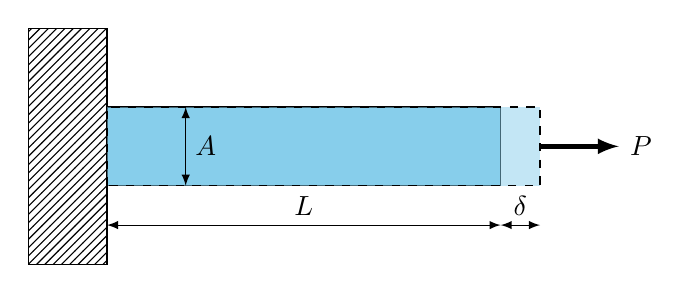
\begin{tikzpicture}[>=latex]
    \draw[pattern=north east lines] (-1,-1) rectangle (0,2);
    \draw[fill=SkyBlue] (0,0) rectangle (5,1);
    \draw[fill=SkyBlue, fill opacity=0.5, dashed] (0,0) rectangle (5.5,1);
    \draw[->,ultra thick] (5.5,0.5) -- (6.5,0.5) node[right]{$P$};
    \draw[<->] (0,-0.5) -- (2.5,-0.5) node[above]{$L$} -- (5,-0.5);
    \draw[<->] (5,-0.5)-- (5.25,-0.5) node[above]{$\delta$} -- (5.5,-0.5);
    \draw[<->] (1,0) -- (1, 0.5) node[right]{$A$} -- (1,1);
  \end{tikzpicture}
\end{figure}
\normalcolor
\begin{align*}
  \sigma  &= \dfrac{P}{A}\\
  \delta  &= \dfrac{PL}{AE}
\end{align*}
\end{frame}

\begin{frame}[label={sec:orgd096fba}]{Critical Location}
\begin{figure}[h]
  \centering
  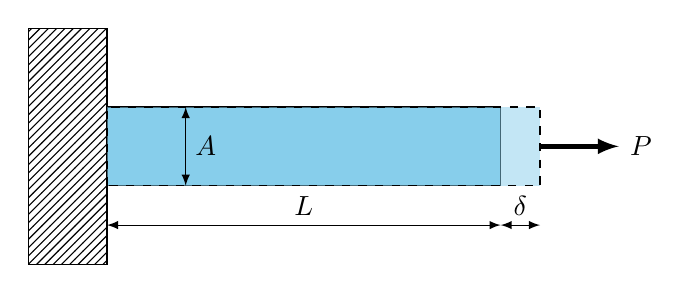
\begin{tikzpicture}[>=latex]
    \draw[pattern=north east lines] (-1,-1) rectangle (0,2);
    \draw[fill=SkyBlue] (0,0) rectangle (5,1);
    \draw[fill=SkyBlue, fill opacity=0.5, dashed] (0,0) rectangle (5.5,1);
    \draw[->,ultra thick] (5.5,0.5) -- (6.5,0.5) node[right]{$P$};
    \draw[<->] (0,-0.5) -- (2.5,-0.5) node[above]{$L$} -- (5,-0.5);
    \draw[<->] (5,-0.5)-- (5.25,-0.5) node[above]{$\delta$} -- (5.5,-0.5);
    \draw[<->] (1,0) -- (1, 0.5) node[right]{$A$} -- (1,1);
  \end{tikzpicture}
\end{figure}
\normalcolor
Where is the critical point for axially loaded members?
\end{frame}

\begin{frame}[label={sec:org397c3a8}]{Bending}
\begin{figure}[h]
  \centering
  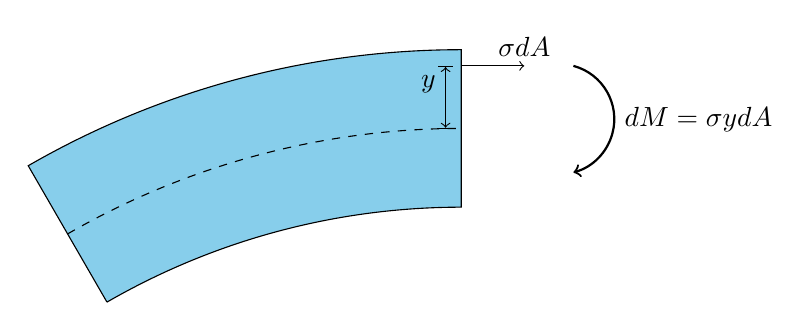
\begin{tikzpicture}
    \draw [fill=SkyBlue] (0,0) arc [radius=9, start angle=120, end angle=90] --
    ++(90:2) arc [radius=11, start angle=90, end angle=120] -- (0,0);
    \draw[dashed, thin] (-0.5,0.866) arc (120:90:10cm);
    \foreach \x in {1}
    \draw[->] (4.5,3.2 - 0.2*\x) -- ++(0: 1-0.2*\x) node(B){} node[above]{$\sigma dA$};
    \draw[->, thick] (B.east) ++ (0:0.5) arc (75:-75:0.7) node[midway, right]{$dM = \sigma y dA$};
    \draw[|<->|] (4.3,2.2) -- (4.3, 3.0) node[below left]{$y$};
  \end{tikzpicture}
\end{figure}
\normalcolor
\begin{align*}
  \sigma = \frac{My}{I}
\end{align*}
\end{frame}

\begin{frame}[label={sec:orgdfbf673}]{Critical Location}
From equation \(\sigma = \dfrac{My}{I}\), where is the critical point?
\begin{figure}[h]
  \centering
  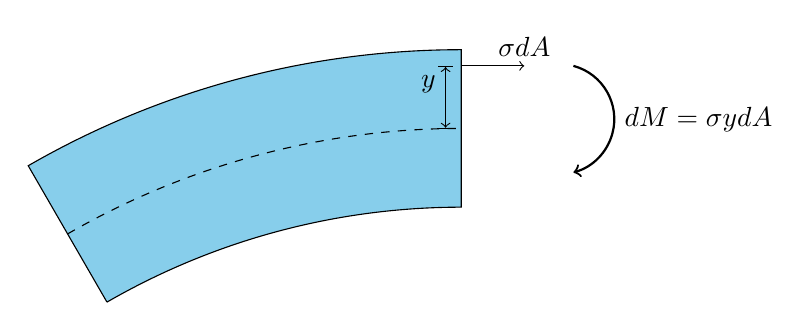
\begin{tikzpicture}
    \draw [fill=SkyBlue] (0,0) arc [radius=9, start angle=120, end angle=90] --
    ++(90:2) arc [radius=11, start angle=90, end angle=120] -- (0,0);
    \draw[dashed, thin] (-0.5,0.866) arc (120:90:10cm);
    \foreach \x in {1}
    \draw[->] (4.5,3.2 - 0.2*\x) -- ++(0: 1-0.2*\x) node(B){} node[above]{$\sigma dA$};
    \draw[->, thick] (B.east) ++ (0:0.5) arc (75:-75:0.7) node[midway, right]{$dM = \sigma y dA$};
    \draw[|<->|] (4.3,2.2) -- (4.3, 3.0) node[below left]{$y$};
  \end{tikzpicture}
\end{figure}
\end{frame}

\begin{frame}[label={sec:orgb6b1824}]{Deflection Analysis}
\centering
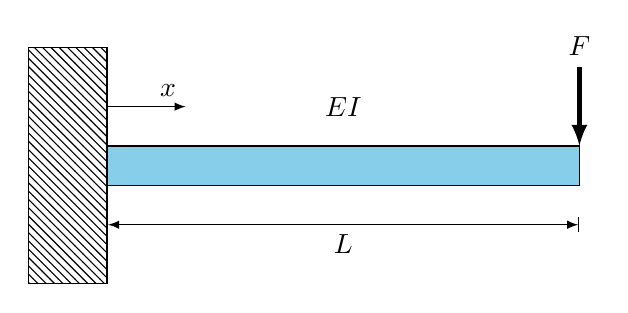
\begin{tikzpicture}[>=latex]
  \draw (0,-0.5) rectangle (1,2.5);
  \fill[pattern=north west lines] (0,-0.5) rectangle (1,2.5);
  \draw[fill=SkyBlue] (1,0.75) rectangle (7,1.25);
  \draw[<-, ultra thick] (7,1.25) -- ++(90:1) node[above]{$F$};
  \draw[|<->|] (1, 0.25) -- (4,0.25) node[below]{$L$} --  (7, 0.25);
  \draw (4,1.75) node{$EI$};
  \draw[->] (1,1.75) -- (2,1.75) node[above left]{$x$};
\end{tikzpicture}
\normalcolor
\begin{equation*}
  \delta = k \frac{FL^3}{EI}
\end{equation*}
\end{frame}

\begin{frame}[label={sec:orgd3caad0}]{Transverse Shear}
\begin{figure}[h]
  \centering
  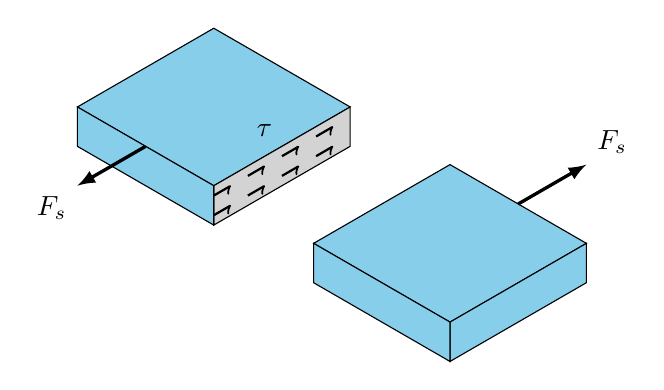
\begin{tikzpicture}[scale=1,>=latex]
    % top left piece
    \draw [fill=SkyBlue] (0,0) -- ++ (30:2) --++ (150:2) --++ (-150:2) node[midway](C){} --cycle node[midway](A){};
    \draw [fill=LightGrey] (0,0) -- ++ (30:2) --++ (-90:0.5) --++ (-150:2) --cycle;
    \draw [fill=SkyBlue] (0,0) -- ++ (150:2) --++ (-90:0.5) --++ (-30:2) --cycle;
    % bottom right piece
    \draw [fill=SkyBlue, xshift=3cm, yshift=-2*0.866cm] (0,0) -- ++ (30:2) node[midway](D){} --++ (150:2) node[midway](B){} --++ (-150:2) --cycle;
    \draw [fill=SkyBlue, xshift=3cm, yshift=-2*0.866cm] (0,0) -- ++ (30:2) --++ (-90:0.5) --++ (-150:2) --cycle;
    \draw [fill=SkyBlue, xshift=3cm, yshift=-2*0.866cm] (0,0) -- ++ (150:2) --++ (-90:0.5) --++ (-30:2) --cycle;
    % shear force pair
    \draw[->, very thick] (A.center) --++ (-150:1) node[below left]{$F_s$};
    \draw[->, very thick] (B.center) --++ (30:1) node[above right]{$F_s$};
    % surface shear stress
    \foreach \x in {0,...,3} {
      \draw[-right to, thick] (0, -0.125) ++ (30:0.5*\x) --++ (30:0.25);
      \draw[-right to, thick] (0, -0.375) ++ (30:0.5*\x) --++ (30:0.25);
    }
    \draw (0,0) ++ (30:1) node[above left]{$\tau$};
  \end{tikzpicture}
  \normalcolor
  \begin{align*}
    \tau = \frac{F}{A}
  \end{align*}
\end{figure}
\end{frame}

\begin{frame}[label={sec:orgeb84f85}]{Torsion}
\begin{figure}[h]
  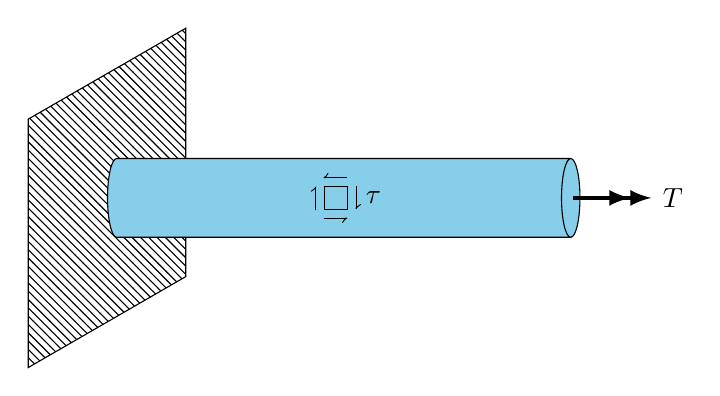
\begin{tikzpicture}[>=latex]
    \node [draw, trapezium, trapezium left angle=120, trapezium right angle=60, minimum height=2cm, minimum width=2cm, rotate=90, pattern=north west lines](wall){};
    \node [anchor=west, draw, fill=SkyBlue, cylinder, minimum height=6cm, minimum width=1cm](bar){};
    \draw [->>, ultra thick] (bar.east) ++ (180:0.1) --++ (0:1) node[right]{$T$};
    \node at (bar.center) [draw, rectangle, minimum height=0.3cm, minimum width=0.3cm](element){};
    \draw [right to-] (element.north west) ++ (90:0.1) --++ (0:0.3);
    \draw [-right to] (element.south west) ++ (-90:0.1) --++ (0:0.3);
    \draw [-left to] (element.south west) ++ (180:0.1) --++ (90:0.3);
    \draw [-left to] (element.north east) ++ (0:0.1) --++ (-90:0.3) node[midway, right]{$\tau$};
  \end{tikzpicture}
\end{figure}
\normalcolor
\begin{align*}
  \tau &= \frac{Tr}{J}
\end{align*}
\end{frame}

\begin{frame}[label={sec:orgb022cc2}]{Critical Location}
\begin{figure}[h]
   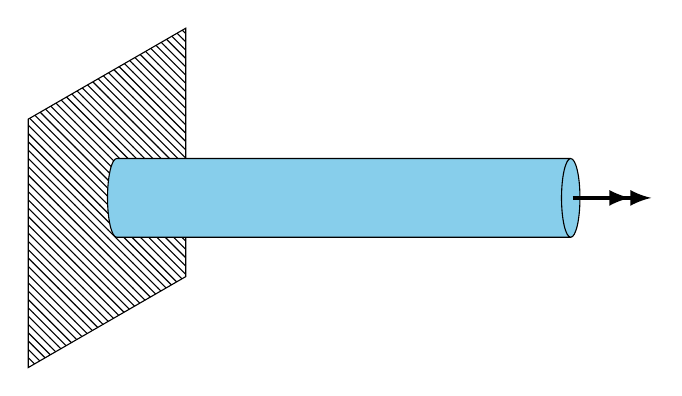
\begin{tikzpicture}[>=latex]
     \node [draw, trapezium, trapezium left angle=120, trapezium right angle=60, minimum height=2cm, minimum width=2cm, rotate=90, pattern=north west lines](wall){};
     \node [anchor=west, draw, fill=SkyBlue, cylinder, minimum height=6cm, minimum width=1cm](bar){};
     \draw [->>, ultra thick] (bar.east) ++ (180:0.1) --++ (0:1);
   \end{tikzpicture}
 \end{figure}
  \normalcolor
Where is the critical location?
\end{frame}

\begin{frame}[label={sec:org886afd7}]{Angle of Twist}
\centering
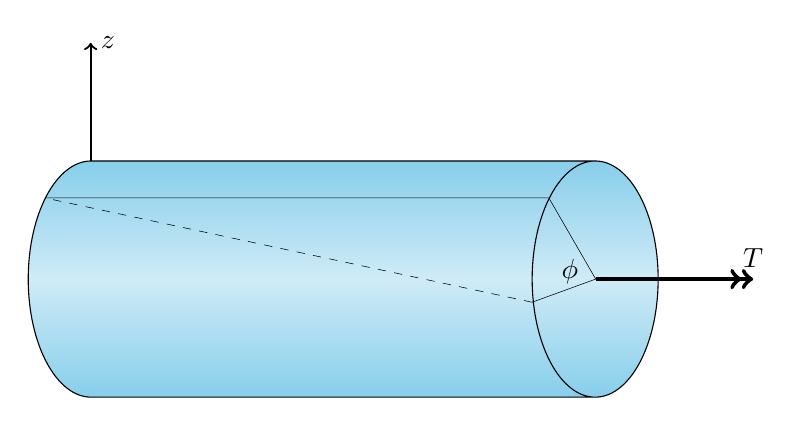
\begin{tikzpicture}
  \draw [->, thick] (0,0) --++ (90:3) node[right]{$z$};
  \node at (0,0) [anchor=west, xshift=-8mm, draw, top color=SkyBlue, bottom color=SkyBlue, middle color=SkyBlue!40, cylinder, minimum height=8cm, minimum width=3cm, inner sep=0.8cm](cyl){};
  \draw [->>, ultra thick] (cyl.east) ++ (180:0.8) node(O){} --++ (0:2) node[above]{$T$};
  \draw [very thin] (O.center) --++ (120:1.19) --++ (180:6.4) node(A){};
  \draw [very thin] (O.center) --++ (200:0.86) node(B){};
  \draw [very thin, dashed] (B.center) -- (A.center);
  \node at (O.center) [left, yshift=1mm, xshift=-1mm] {$\phi$};
\end{tikzpicture}
\normalcolor
\begin{equation}
  \phi = \frac{TL}{GJ}
\end{equation}
\end{frame}

\begin{frame}[label={sec:orgfb744ff}]{Contact}
\begin{figure}[h]
  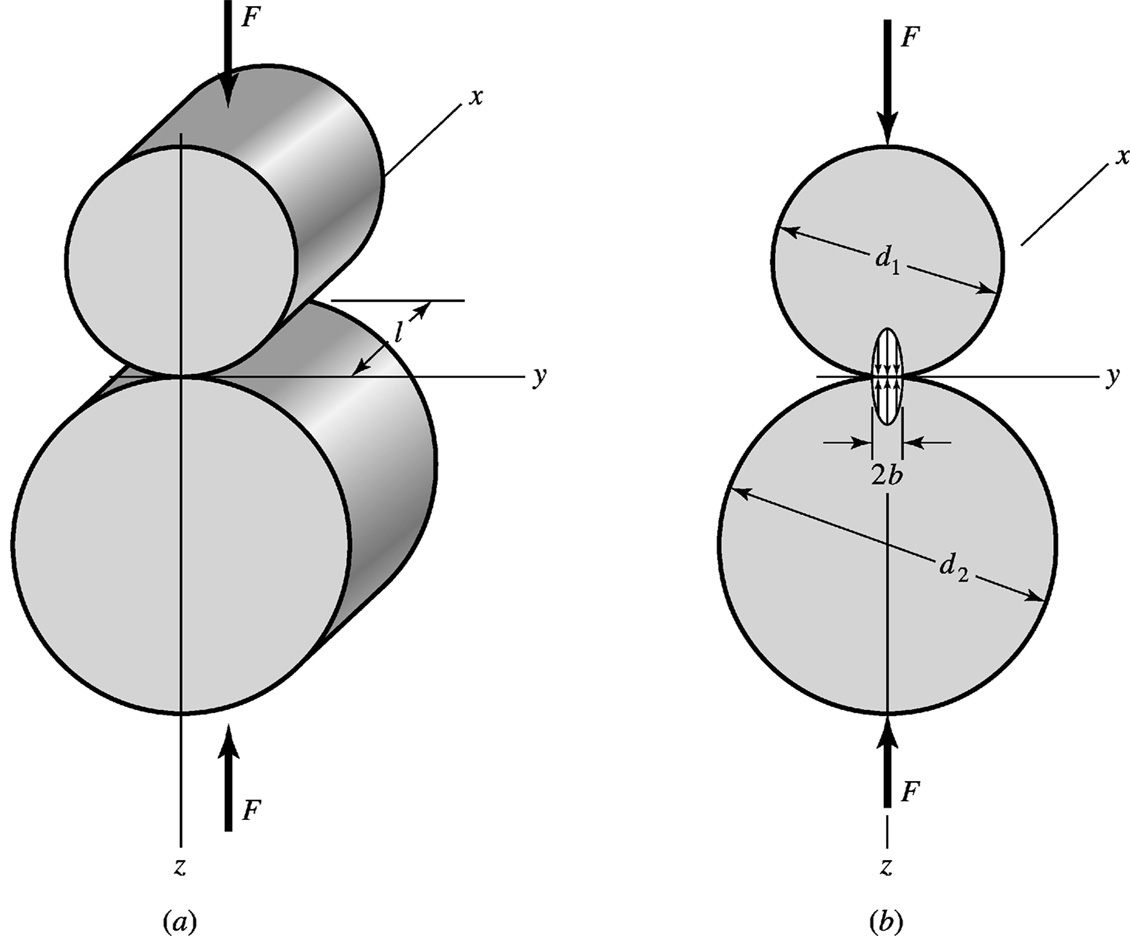
\includegraphics[scale=0.5]{pictures/contact-stress}
\end{figure}
\begin{align*}
  \sigma_{avg} &= \frac{F}{A} = \frac{F}{2bl}
\end{align*}
\end{frame}


\section{Multiaxial Analysis}
\label{sec:orga962368}
\begin{frame}[label={sec:orgede3d3b}]{Stress Transformation}
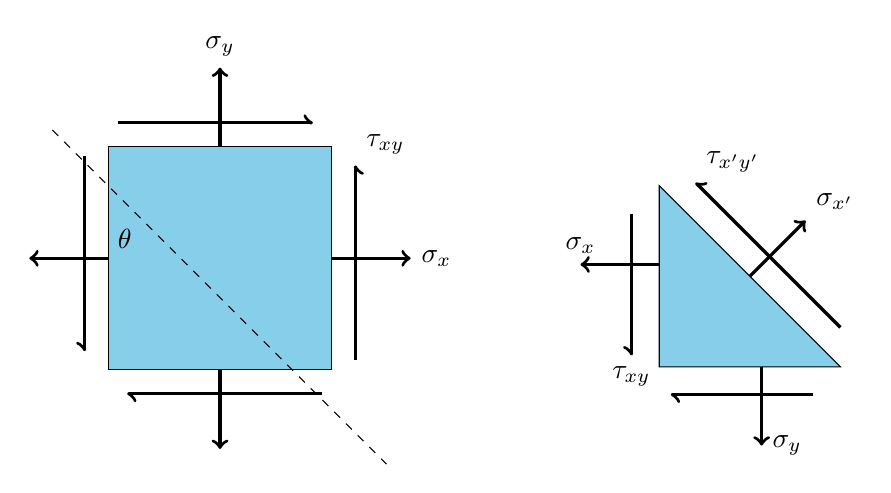
\begin{tikzpicture}
  \node [draw, fill=SkyBlue, regular polygon, regular polygon sides=4, minimum width=4cm](A){};
  \draw [->,very thick] (A.north) --++ (90:1) node[above]{$\sigma_y$};
  \draw [->,very thick] (A.east) --++ (0:1) node[right]{$\sigma_x$};
  \draw [->,very thick] (A.west) --++ (180:1);
  \draw [->,very thick] (A.south) --++ (-90:1);
  \node at (A.north west) [yshift=3mm] (B){};
  \draw [-left to, very thick] (B) --++ (0:2.6);
  \node at (A.south east) [xshift=3mm] (C){};
  \draw [-right to, very thick] (C) --++ (90:2.6) node[above right]{$\tau_{xy}$};
  \node at (A.north west) [xshift=-3mm] (D){};
  \draw [-right to, very thick] (D) --++ (-90:2.6);
  \node at (A.south east) [yshift=-3mm] (E){};
  \draw [-left to, very thick] (E) --++ (180:2.6);
  \draw [dashed] (A.north west) ++ (-90:0.5) node(F){} ++ (135:1) --++ (-45:6);
  \node at (A.west) [above right]{$\theta$};
  \draw [fill=SkyBlue] (F) ++ (0:7) node(G){} --++ (-90:2.3) node(H){} --++ (0:2.3) node(I){} -- cycle node[midway](J){};
  \draw [->, very thick] (G.center) ++ (-90:1) --++ (180:1) node[above]{$\sigma_x$};
  \draw [->, very thick] (H.center) ++ (0:1.3) --++ (-90:1) node[right]{$\sigma_y$};
  \draw [-left to, very thick] (I.center) ++ (-135:0.5) --++ (180:1.8);
  \draw [-right to, very thick] (G.center) ++ (-135:0.5) --++ (-90:1.8) node[below]{$\tau_{xy}$};
  \draw [->, very thick] (J.center) --++ (45:1) node[above right]{$\sigma_{x'}$};
  \draw [-right to, very thick] (I.center) ++ (90:0.5) --++ (135:2.6) node[above right]{$\tau_{x'y'}$};
\end{tikzpicture}
\end{frame}

\begin{frame}[label={sec:org38f2906}]{Principal and Maximum Shear Stresses}
\begin{columns}
\begin{column}{0.5\columnwidth}
\scriptsize
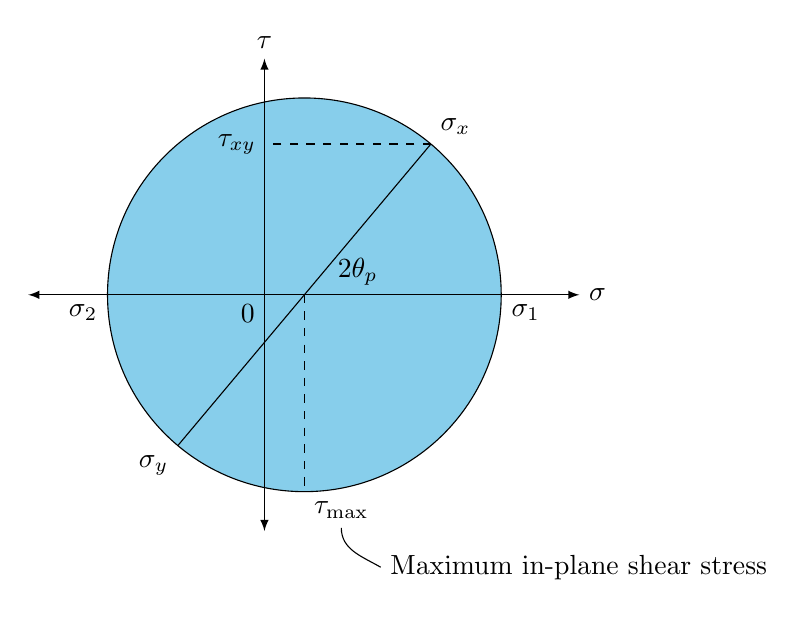
\begin{tikzpicture}[>=latex]
  \node at (-2,0) [anchor=west, draw, fill=SkyBlue, circle, minimum height=5cm](large){};
  \draw [<->] (-3,0) --++ (0:7) node[right]{$\sigma$};
  \draw [<->] (0,-3) --++ (90:6) node[above]{$\tau$};
  \node at (large.east) [below right] {$\sigma_1$};
  \node at (large.west) [below left] {$\sigma_2$};
  \draw (0,0) node[below left]{0};
  \draw [dashed](large.center) -- (large.south) node[below right](absolute){$\tau_{\max}$};
  \draw (large.center) --++ (50:2.5) node[above right]{$\sigma_x$} node(A){};
  \draw (large.center) --++ (-130:2.5) node[below left]{$\sigma_y$};
  \draw [dashed] (A.center) --++ (180:2.1) node[left]{$\tau_{xy}$};
  \draw (absolute.south) [out=-90, in=150] to ++(0.5,-0.5) node[right]{Maximum in-plane shear stress};
  \node at (large.center) [above right, xshift=3mm] {$2\theta_p$};
\end{tikzpicture}
\end{column}

\begin{column}{0.5\columnwidth}
\normalsize
\begin{gather*}
  \sigma_{1,2} = \frac{\sigma_x + \sigma_y}{2} \pm \sqrt {\frac{\sigma_x - \sigma_y}{2}^2 + \tau_{xy}^2} \\[10pt]
  \tau_{\max} = \sqrt {\left( \frac{\sigma_x - \sigma_y}{2} \right)^2 + \tau_{xy}^2} \\[10pt]
  \tan 2\theta_p = \frac{2 \tau_{xy}}{\sigma_x - \sigma_y}
\end{gather*}
\vspace{2cm}
\end{column}
\end{columns}
\end{frame}

\begin{frame}[label={sec:org0a02607}]{Determining Critical Location}
\begin{itemize}
\item Determine critical points resulting from individual loads
\item Find coincident critical points
\item Check if there are any reinforcing or canceling stresses
\end{itemize}
\end{frame}

\begin{frame}[label={sec:org828dc4c}]{Example: Shaft under multiple loads}
\begin{figure}[htbp]
  \centering
  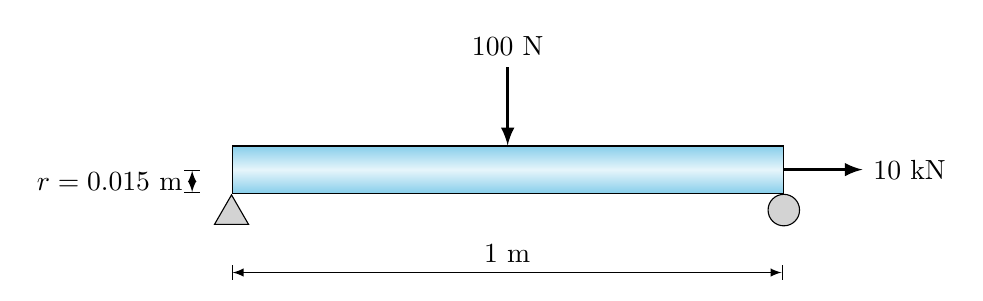
\begin{tikzpicture}[>=latex]
    \node [draw, top color=SkyBlue, bottom color=SkyBlue, middle color=SkyBlue!20, minimum height=6mm, minimum width=7cm](beam){};
    % supports
    \node at (beam.south east) [anchor=north, draw, fill=LightGrey, circle, minimum height=4mm, inner sep=0] (B){};
    \node at (beam.south west) [anchor=north, draw, fill=LightGrey, regular polygon, regular polygon sides=3, minimum height=5mm, inner sep=0] {};
    % dimensions
    \draw [|<->|] (beam.south west) ++ (-90:1) --++ (0:7) node[midway, above]{1 m};
    \draw [|<->|] (beam.west) ++ (180:0.5) --++ (-90:0.3) node[midway, left]{$r = 0.015$ m};
    % loads
    \draw [<-, very thick] (beam.north) --++ (90:1) node[above]{100 N};
    \draw [->, very thick] (beam.east) --++ (0:1) node[right]{10 kN};
  \end{tikzpicture}
\end{figure}

\normalcolor
Determine the critical point location and its state of stress.
\end{frame}

\begin{frame}[label={sec:org5aa8ac5}]{Solution}
\begin{itemize}
\item Determine critical points from individual loads
\end{itemize}

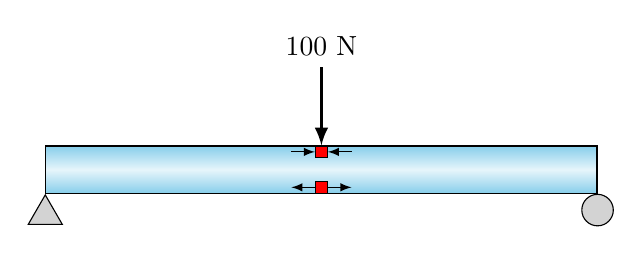
\begin{tikzpicture}[>=latex]
  \node [draw, top color=SkyBlue, bottom color=SkyBlue, middle color=SkyBlue!20, minimum height=6mm, minimum width=7cm](beam){};
  % supports
  \node at (beam.south east) [anchor=north, draw, fill=LightGrey, circle, minimum height=4mm, inner sep=0] (B){};
  \node at (beam.south west) [anchor=north, draw, fill=LightGrey, regular polygon, regular polygon sides=3, minimum height=5mm, inner sep=0] {};
  \node at (beam.south) [anchor=south, draw, fill=red, rectangle, minimum height=1.5mm, minimum width=1.5mm, inner sep=0](critsouth){};
  \node at (beam.north) [anchor=north, draw, fill=red, rectangle, minimum height=1.5mm, minimum width=1.5mm, inner sep=0](critnorth){};
  \draw [<-] (critnorth.west) --++ (180:0.3);
  \draw [<-] (critnorth.east) --++ (0:0.3);
  \draw [->] (critsouth.west) --++ (180:0.3);
  \draw [->] (critsouth.east) --++ (0:0.3);
  % loads
  \draw [<-, very thick] (beam.north) --++ (90:1) node[above]{100 N};
\end{tikzpicture}
\end{frame}

\begin{frame}[label={sec:org4fc092a}]{Determining Critical Location}
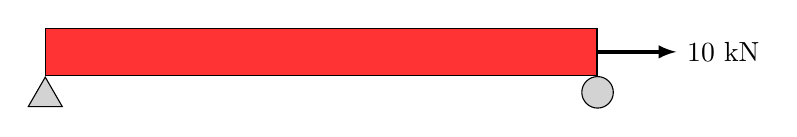
\begin{tikzpicture}[>=latex]
  \node [draw, fill=red!80, minimum height=6mm, minimum width=7cm](beam){};
  % supports
  \node at (beam.south east) [anchor=north, draw, fill=LightGrey, circle, minimum height=4mm, inner sep=0] (B){};
  \node at (beam.south west) [anchor=north, draw, fill=LightGrey, regular polygon, regular polygon sides=3, minimum height=5mm, inner sep=0] {};
  \draw [->, very thick] (beam.east) --++ (0:1) node[right]{10 kN};
\end{tikzpicture}

The common spots are top and bottom middle. Once taking directions of stresses into account, the bottom middle element is clearly the critical point.

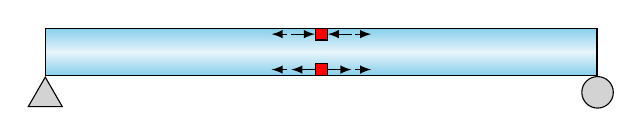
\begin{tikzpicture}[>=latex]
  \node [draw, top color=SkyBlue, bottom color=SkyBlue, middle color=SkyBlue!20, minimum height=6mm, minimum width=7cm](beam){};
  % supports
  \node at (beam.south east) [anchor=north, draw, fill=LightGrey, circle, minimum height=4mm, inner sep=0] (B){};
  \node at (beam.south west) [anchor=north, draw, fill=LightGrey, regular polygon, regular polygon sides=3, minimum height=5mm, inner sep=0] {};
  \node at (beam.south) [anchor=south, draw, fill=red, rectangle, minimum height=1.5mm, minimum width=1.5mm, inner sep=0](critsouth){};
  \node at (beam.north) [anchor=north, draw, fill=red, rectangle, minimum height=1.5mm, minimum width=1.5mm, inner sep=0](critnorth){};
  \draw [<-] (critnorth.west) --++ (180:0.3);
  \draw [->] (critnorth.west) ++ (180:0.35) --++ (180:0.2);
  \draw [<-] (critnorth.east) --++ (0:0.3);
  \draw [->] (critnorth.east) ++ (0:0.35) --++ (0:0.2);
  \draw [->] (critsouth.west) --++ (180:0.3);
  \draw [->] (critsouth.west) ++ (180:0.35) --++ (180:0.2);
  \draw [->] (critsouth.east) --++ (0:0.3);
  \draw [->] (critsouth.east) ++ (0:0.35) --++ (0:0.2);
\end{tikzpicture}
\end{frame}

\begin{frame}[label={sec:orgad159b3}]{Solution: Determining Critical Location}
To determine the state of stress, we must first determine resultant stresses from axial load and bending. For axial load, we have

\begin{align*}
\sigma_a &= \frac{F}{A} \\
&= \frac{10000}{\pi (0.015)^2} \\
&= 14.15 \text{ MPa}
\end{align*}
\end{frame}

\begin{frame}[label={sec:org5ab35e2}]{Solution: Determining Critical Solution}
For bending, we have
\begin{align*}
\sigma_b &= \frac{My}{I} \\
&= \frac{100(1)(0.015)}{4 \dfrac{\pi}{4}(0.015)^4} \\
&= 9.43 \text{ MPa}
\end{align*}

\begin{figure}[h]
  \centering
  \begin{tikzpicture}[>=latex]
    \node at (beam.south) [anchor=south, draw, fill=red, rectangle, minimum height=5mm, minimum width=5mm, inner sep=0](critsouth){};
    \draw [->] (critsouth.west) --++ (180:0.5);
    \draw [->] (critsouth.west) ++ (180:0.55) --++ (180:0.4);
    \draw [->] (critsouth.east) --++ (0:0.5);
    \draw [->] (critsouth.east) ++ (0:0.55) --++ (0:0.4);
  \end{tikzpicture}
\end{figure}

\(\sigma_{total} = 14.15 + 9.43\) = 23.58 MPa.
\end{frame}

\begin{frame}[label={sec:org587bb09}]{Exercise: Combined Loadings}
\centering
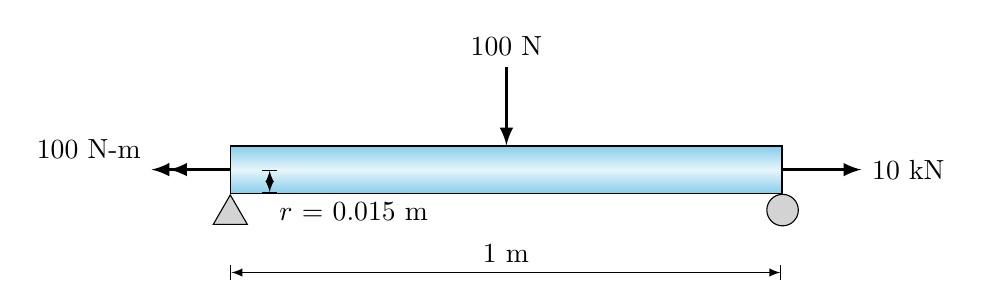
\begin{tikzpicture}[>=latex]
  \node [draw, top color=SkyBlue, bottom color=SkyBlue, middle color=SkyBlue!20, minimum height=6mm, minimum width=7cm](beam){};
  % supports
  \node at (beam.south east) [anchor=north, draw, fill=LightGrey, circle, minimum height=4mm, inner sep=0] (B){};
  \node at (beam.south west) [anchor=north, draw, fill=LightGrey, regular polygon, regular polygon sides=3, minimum height=5mm, inner sep=0] {};
  % dimensions
  \draw [|<->|] (beam.south west) ++ (-90:1) --++ (0:7) node[midway, above]{1 m};
  \draw [|<->|] (beam.west) ++ (0:0.5) --++ (-90:0.3) node[below right]{$r$ = 0.015 m};
  % loads
  \draw [<-, very thick] (beam.north) --++ (90:1) node[above]{100 N};
  \draw [->, very thick] (beam.east) --++ (0:1) node[right]{10 kN};
  \draw [->>, very thick] (beam.west) --++ (180:1) node[above left]{100 N-m};
\end{tikzpicture}

\begin{itemize}
\item Determine the critical point
\item Determine the state of stress at the critical point
\item Find the principal stresses and principal direction at the critical point
\end{itemize}
\end{frame}





\section{Failure of Materials}
\label{sec:org3986e69}
\begin{frame}[label={sec:org1f05f62}]{Failure}
\begin{enumerate}
\item Yield \& Fracture
\item Fatigue
\item Buckling
\end{enumerate}
\end{frame}

\begin{frame}[label={sec:org2989aca}]{Fracture \& Yield}
\begin{itemize}
\item Sufficiently high stress to overcome intermolecular bonds
\item Under uniaxial stress, a material fails when

\begin{itemize}
\item Brittle material - broken molecular bond leads to material separation --  \alert{Fracture}
\item Ductile material - surface slip -- \alert{Yield}
\end{itemize}
\end{itemize}
\end{frame}

\begin{frame}[label={sec:orgc4ff6c3}]{Design Equation for MNST}
\begin{columns}
\begin{column}{0.4\columnwidth}
if \(\sigma_1 > \sigma_2\)
$$ \sigma_1 = \frac{S_{ut}}{N_s} $$
$$ \sigma_2 = \frac{S_{uc}}{N_s} $$
\end{column}
\begin{column}{0.6\columnwidth}
\begin{tikzpicture}[>=latex]
  \node [draw, rectangle, xshift=-1cm, yshift=-1cm, minimum height=4cm, minimum width=4cm](sq){};
  \node [draw, rectangle, xshift=-0.5cm, yshift=-0.5cm, minimum height=4cm, minimum width=4cm, scale=0.5, dashed]{};
  \node [draw, rectangle, xshift=-.33cm, yshift=-.33cm, minimum height=4cm, minimum width=4cm, scale=0.33, dashed]{};
  \draw [<->] (-4,0) --++ (0:6) node[right]{$\sigma_1$};
  \node at (sq.east) [yshift=7mm, right] {$S_{ut}$};
  \node at (sq.west) [yshift=7mm, left] {$S_{uc}$};
  \node at (sq.north) [xshift=1.3cm, above] {$S_{ut}$};
  \node at (sq.south) [xshift=7mm, below] {$S_{uc}$};
  \draw [<->] (0,-4) --++ (90:6) node[above]{$\sigma_2$};
\end{tikzpicture}
\end{column}
\end{columns}
\end{frame}

\begin{frame}[label={sec:org17513ef}]{Design Equation for MSST}
\begin{columns}
\begin{column}{0.2\columnwidth}
\begin{gather*}
  \tau_{max} = \frac{S_y}{2N_s} \\
  \sigma_{1,2} = \frac{S_y}{N_s}
\end{gather*}
\end{column}

\begin{column}{0.5\columnwidth}
\begin{tikzpicture}[>=latex, scale=0.8]
  \draw [dashed] (0,-3) node[right]{$-S_y$} -- (3,0) node[below right]{$S_y$} -- (3,3) -- (0,3) node[midway, below]{\footnotesize{$N_{s} = 1$}} node[left]{$S_y$} -- (-3,0) node[above left]{$-S_y$} -- (-3,-3) -- cycle;
  \draw [dashed, scale=0.5] (0,-3) node[right]{} -- (3,0) node[below right]{} -- (3,3) -- (0,3) node[midway, below]{\footnotesize{2}} node[left]{} -- (-3,0) node[above left]{} -- (-3,-3) -- cycle;
  \draw [dashed, scale=0.33] (0,-3) node[right]{} -- (3,0) node[below right]{} -- (3,3) -- (0,3) node[midway, below]{\footnotesize{3}} node[left]{} -- (-3,0) node[above left]{} -- (-3,-3) -- cycle;
  \draw [<->] (-4,0) --++ (0:8) node[right]{$\sigma_1$};
  \draw [<->] (0,-4) --++ (90:8) node[above]{$\sigma_2$};
\end{tikzpicture}
\end{column}
\end{columns}
\end{frame}

\begin{frame}[label={sec:org2f21ffd}]{Design Equation for MDET}
\begin{columns}
\begin{column}{0.4\columnwidth}
$$ \sigma_e = \frac{S_y}{N_s} $$
\end{column}
\begin{column}{0.6\columnwidth}
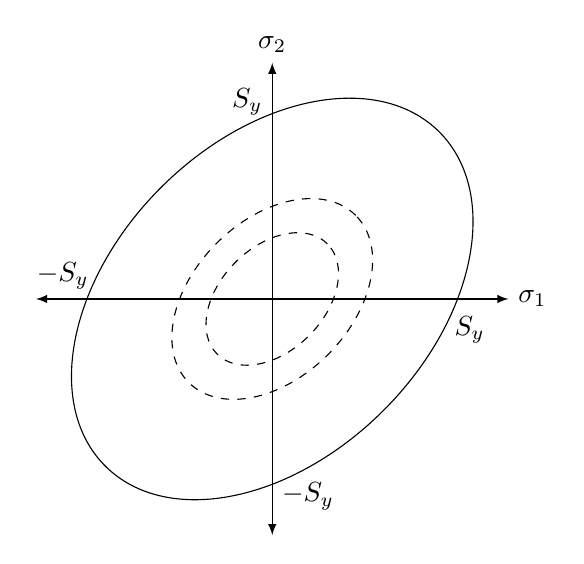
\begin{tikzpicture}[>=latex]
  \node [draw, ellipse, minimum width=6cm, minimum height=4cm, rotate=45](el){};
  \node [draw, ellipse, minimum width=6cm, minimum height=4cm, rotate=45, scale=0.5, dashed]{};
  \node [draw, ellipse, minimum width=6cm, minimum height=4cm, rotate=45, scale=0.33, dashed]{};
  \node at (el.north east)[left, xshift=-5mm]{$S_y$};
  \node at (el.south east)[below, yshift=-6mm]{$S_y$};
  \node at (el.north west)[above left, yshift=5mm, xshift=3mm]{$-S_y$};
  \node at (el.south west)[right, xshift=5mm]{$-S_y$};
  \draw [<->] (-3,0) --++ (0:6) node[right]{$\sigma_1$};
  \draw [<->] (0,-3) --++ (90:6) node[above]{$\sigma_2$};
\end{tikzpicture}
\end{column}
\end{columns}
\end{frame}

\begin{frame}[label={sec:orgebfff61}]{Fatigue Equations}
\begin{itemize}
\item Soderberg relation
$$ \dfrac{\sigma_a}{S_e} + \dfrac{\sigma_m}{S_y} = \dfrac{1}{N_s} $$
\item Gerber relation
$$ \dfrac{\sigma_a}{S_e} + \left( \dfrac{\sigma_m}{S_{ut}} \right)^2 = \dfrac{1}{N_s} $$
\item Goodman relation
$$ \dfrac{\sigma_a}{S_e} + \dfrac{\sigma_m}{S_{ut}} = \dfrac{1}{N_s} $$
\end{itemize}


These are called \emph{constant life lines}.
\end{frame}

\begin{frame}[label={sec:org29bf11e}]{Buckling}
\begin{itemize}
\item Instability of column under compressive load
\end{itemize}

\vspace{3mm}
$$ P = \dfrac{n^2 \pi^2 E I}{L^2} \hspace{1cm}n = 1, 2, \ldots $$
\end{frame}

\begin{frame}[label={sec:orgfd6ae3a}]{Critical Load and Corresponding Mode Shape}
For \(n = 1\)
   $$ P_{crit} = \dfrac{\pi^2 E I}{L^2} $$
This is called \emph{Euler load} or \emph{Critical load}. \\\empty
\vspace{5mm}
What does the corresponding buckled column look like?
   $$ v(x) = B \sin \sqrt{\frac{P}{EI}} \, x = B \sin \dfrac{n \pi x}{L} $$
\end{frame}

\begin{frame}[label={sec:org19f1008}]{Generalized Critical Load}
\begin{align*}
  P_{cr} &= \frac{\pi^2 EI}{L_e^2} \\
       L_e &= KL
\end{align*}
\begin{align*}
  L_e &= \text{effective length} \\
  K &= \text{constant depending on supports}
\end{align*}
\end{frame}

\begin{frame}[label={sec:orgbefdd62}]{Buckling Design Equation}
\begin{align*}
  P_{allow} = \frac{P_{cr}}{N_{s}} &= \frac{\pi^2 EI}{N_{s}L_e^2} \\
  \sigma_{allow} = \frac{\sigma_{cr}}{N_{s}} &= \frac{\pi^2 E}{ N_{s}\lambda^2}
\end{align*}
\end{frame}

\section{Stress Concentration}
\label{sec:org925f0f9}

\begin{frame}[label={sec:orge72df39}]{Theory vs Experiment}
\centering
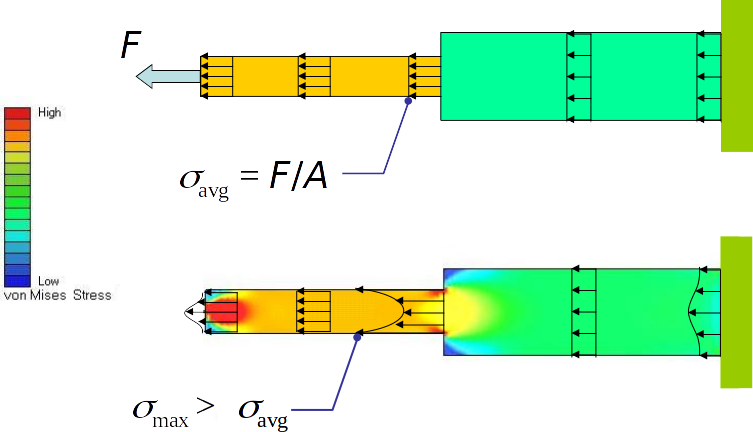
\includegraphics[width=0.9\textwidth]{pictures/theory-experiment}
\end{frame}

\begin{frame}[label={sec:org255b99e}]{Stress Flow}
\centering
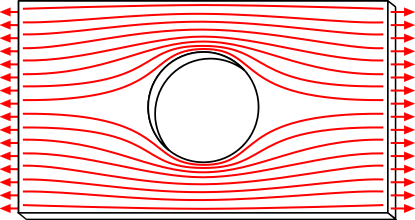
\includegraphics[width=0.8\textwidth]{pictures/force-flow}
\end{frame}

\begin{frame}[label={sec:org8a1357c}]{Good Stress Concentration}
\centering
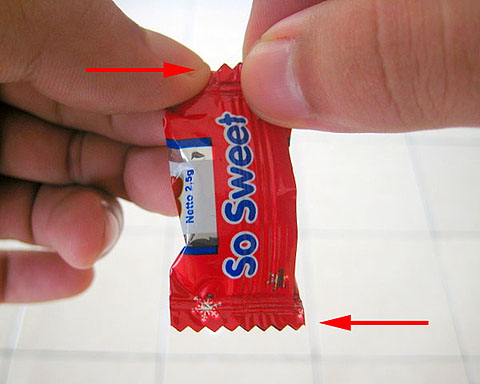
\includegraphics[width=0.8\textwidth]{pictures/good-stress-conc}
\end{frame}

\begin{frame}[label={sec:org13f90da}]{Bad Stress Concentration}
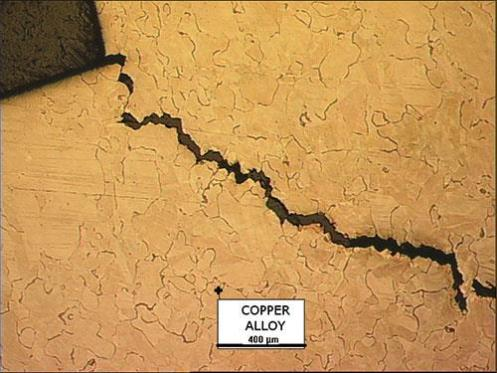
\includegraphics[width=0.49\textwidth]{pictures/copper-concentration}
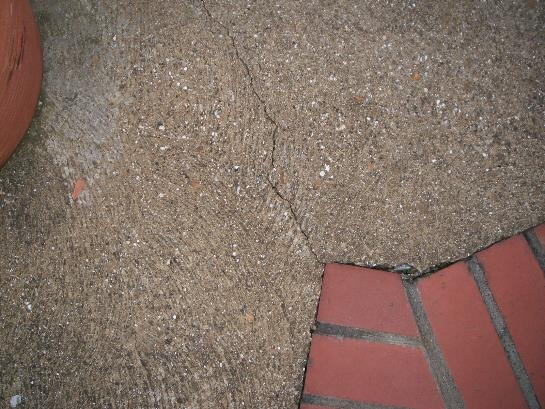
\includegraphics[width=0.49\textwidth]{pictures/concrete-concentration}
\end{frame}

\begin{frame}[label={sec:org651e6fb}]{De Havilland Comet}
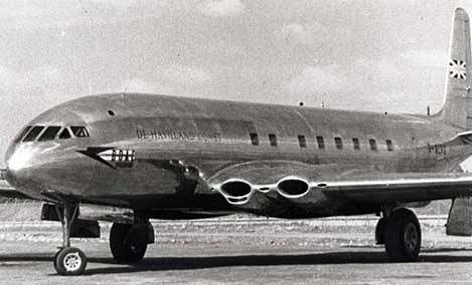
\includegraphics[width=0.49\textwidth]{pictures/airplane-stress-conc}
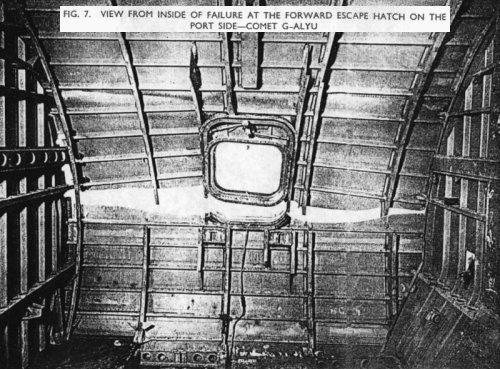
\includegraphics[width=0.49\textwidth]{pictures/airplane-broken-fuselage}


**
  \frametitle{Da Havilland Comet Stress}
  \centering
  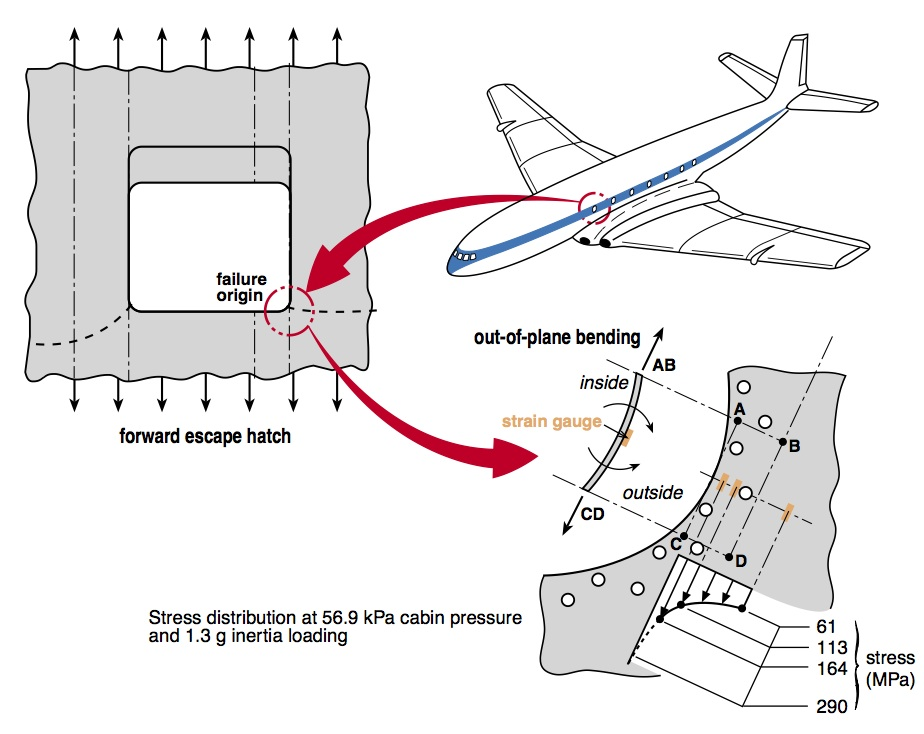
\includegraphics[height=0.87\textheight]{pictures/de-havilland-stress}
\end{frame}

\begin{frame}[label={sec:org0ae8dc9}]{Stress Concentration Factors}
\begin{itemize}
\item Stress concentration factor $K$
  $$ K = \frac{\sigma_{\max}}{\sigma_{\text{avg}}} $$
\item depends on geometry
\end{itemize}
\end{frame}

\begin{frame}[label={sec:org94d0067}]{Photoelastic vs Simulation}
\centering
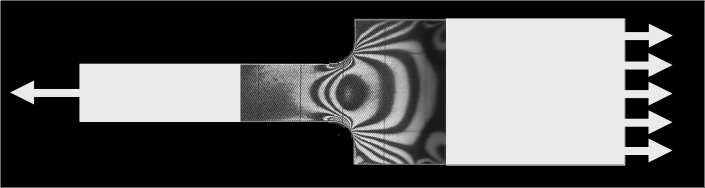
\includegraphics[width=0.7\textwidth]{pictures/photoelasticity} \\\empty
\vspace{5mm}
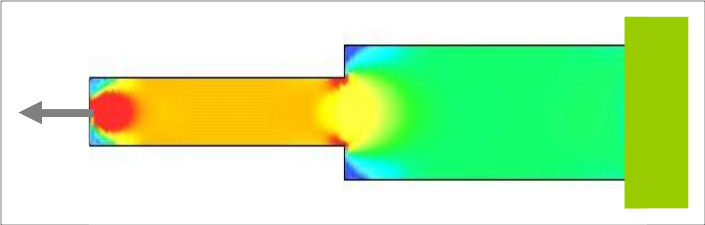
\includegraphics[width=0.7\textwidth]{pictures/simulation}
\end{frame}

\begin{frame}[label={sec:org445ff14}]{Stress Concentration Factor Chart}
\centering
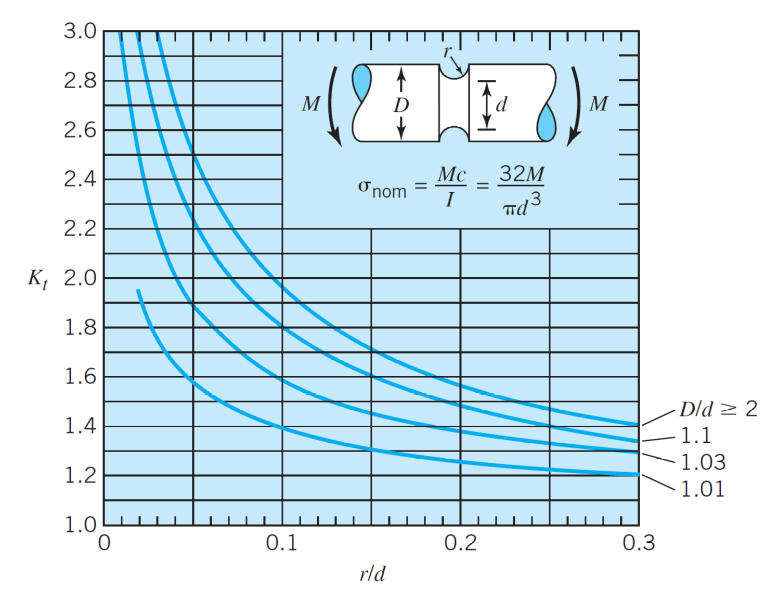
\includegraphics[width=0.8\textwidth]{pictures/stress-conc-grooved-shaft}
\end{frame}

\begin{frame}[label={sec:org3861cf7}]{Example}
Determine the maximum load this multi-segment cantilever beam can take given that the beam material has \(\sigma_{allow}\) = 150 MPa.

\centering
\footnotesize
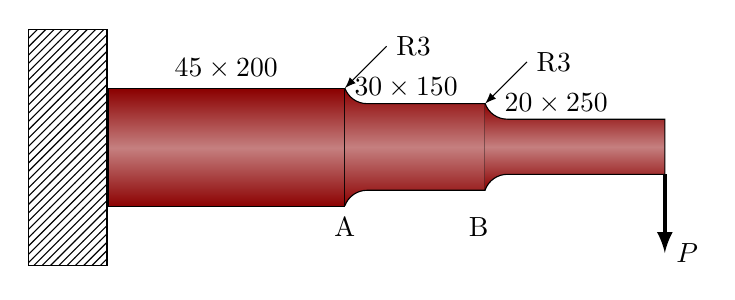
\begin{tikzpicture}[>=latex]
  \node [draw, top color=DarkRed, bottom color=DarkRed, middle color=DarkRed!50!white, rectangle, minimum height=1.5cm, minimum width=3cm](left){};
  \node at (left.west) [anchor=east, draw, pattern=north east lines, minimum height=3cm, minimum width=1cm]{};
  \draw [top color=DarkRed, bottom color=DarkRed, middle color=DarkRed!50!white] (left.north east) arc (-160:-90:0.3) --++ (0:1.5) node(middle){} --++ (-90:1.1) --++ (180:1.5) arc (90:160:0.3);
  \draw [top color=DarkRed, bottom color=DarkRed, middle color=DarkRed!50!white] (middle) arc (-160:-90:0.3) --++ (0:2) --++ (-90:0.7) node(force){} --++ (180:2) arc (90:160:0.3);
  \draw [->, ultra thick] (force.center) --++ (-90:1) node[right]{$P$};
  \draw [<-] (left.north east) --++ (45:0.75) node[right]{R3};
  \draw [<-] (middle.center) --++ (45:0.75) node[right]{R3};
  \node at (left.south east) [below] {A};
  \node at (left.south east) [xshift=1.7cm, below] {B};
  \node at (left.north) [above]{$\diameter 45 \times 200$};
  \node at (left.north east) [right]{$\diameter 30 \times 150$};
  \node at (middle.east) [right]{$\diameter 20 \times 250$};
\end{tikzpicture}
\end{frame}

\begin{frame}[label={sec:orgcafbd61}]{Example: Use this chart}
\centering
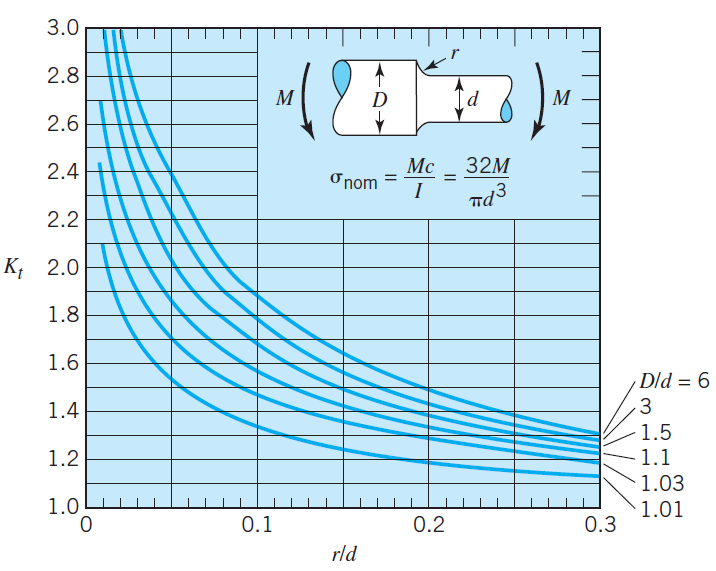
\includegraphics[width=0.8\textwidth]{pictures/stress-conc-shaft-shoulder-fillet-bending}
\end{frame}

\begin{frame}[label={sec:org2cafb2e}]{Avoid Stress Concentration Factor}
\centering
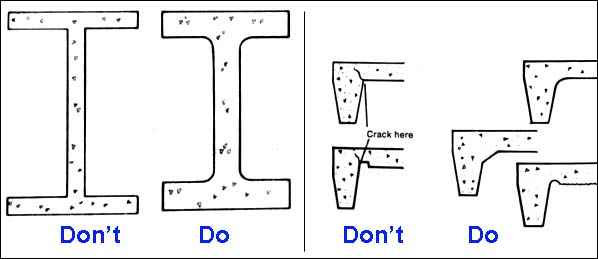
\includegraphics[width=0.6\textwidth]{pictures/avoid-sharp-corners} \\\empty
\vspace{0.3cm}
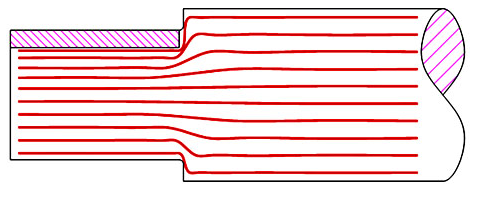
\includegraphics[width=0.45\textwidth]{pictures/avoid-sharp-shoulder}
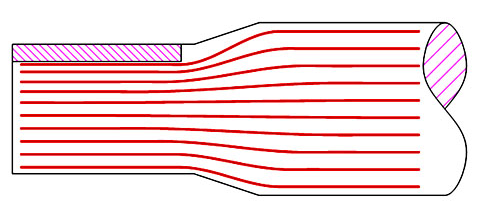
\includegraphics[width=0.45\textwidth]{pictures/avoid-sharp-shoulder2}
\end{frame}
\end{document}